\chapter{Uma Rede de Colaboração para a UnB}

%------------------------------------------------------------------------------%
Como dito anteriormente, o objetivo deste trabalho é disponibilizar um ambiente
virtual na forma de uma rede de colaboração livre para a Universidade de
Brasília. Para isto, escolhemos utilizar a plataforma Noosfero por entender que
esta satisfaz nossas necessidades pelo fato de ser uma plataforma de software
livre, por ser expansível (através de \textit{plugins}), por ter uma comunidade
ativa e pela posição geográfica favorável que possuímos em relação ao núcleo de
desenvolvimento desta, a Colivre, que é uma cooperativa brasileira com sede na
Bahia. Desta forma, conseguimos facilmente contactar os principais desenvolvedores
do Noosfero e organizar encontros para discutir parcerias, como já foi realizado
no \textit{fisl14}~\footnote{Foi realizado um encontro de usuários do Noosfero
no 14º Fórum Internacional de Software Livre, em Porto Alegre - RS 
(\url{}http://softwarelivre.org/noosfero/blog/relato-do-encontro-comunitario-
do-noosfero-no-fisl-14)}.

Queremos que esta rede proposta funcione como um ambiente complementar de ensino
a ser utilizado nas disciplinas de graduação e pós-graduação e nos projetos da
Universidade. Assim, seriam criadas comunidades para estes
que serviriam como um ponto de acesso público aos trabalhos e conteúdos
desenvolvidos pelos alunos que seriam publicados
na comunidade na forma de \textit{posts} em \textit{blogs} ou de artigos de
texto organizados dentro de pastas uma vez que o Noosfero disponibiliza esta
forma de organização de conteúdo.
%
Também é possível criar sub-comunidades para os diversos projetos que
eventualmente possam existir dentro de uma disciplina (caso evidenciado na
sub-seção \ref{mes-unb}) através do \textit{plugin} de sub-comunidades
desenvolvido pela USP como parte do projeto do Stoa.
%
Dentre as vantagens dessa abordagem podemos destacar a possibilidade de acesso
público, uma vez que produzir conhecimento que seja aproveitado pela comunidade
seja uma função de uma Universidade, e a persistência do conteúdo desenvolvido
para as comunidades. A publicidade do conteúdo pode ser configurada através das
permissões de acesso que podem ser alteradas no painel de controle da comunidade.
Em relação à persistência, as comunidades não precisariam ter seu conteúdo
removidos a cada semestre, uma prática comum no uso do Moodle, mas
possibilitariam que outros integrantes da comunidade dessem continuidade à
construção dele de forma evolutiva.

Entendemos que o processo de adoção de uma ferramenta nova para o ensino seja
um processo gradual e que necessite da colaboração do corpo docente para seu
sucesso, além da necessidade de treinamento para seu uso de forma eficaz.
Nesse capítulo apresentamos o estado atual do processo de implantação da rede
de colaboração da UnB e os requisitos para seu funcionamento, além de
apresentarmos um cronograma de trabalho.

%------------------------------------------------------------------------------%

\section{Estado Atual}

O trabalho de implantação desta rede de colaboração conta com o apoio do \\ CDTC
~\footnote{\url{http://comunidade.cdtc.org.br/}}(Centro de Difusão de Tecnologia
e Conhecimento) que tem uma sede localizada no sub-solo do ICC no campus Darcy
Ribeiro. Esta parceria acelerou o processo de implantação de uma instância do
Noosfero (atualmente chamada de Comunidade UnB) em um ambiente de
testes~\footnote{Disponível em \url{http://comunidade.unb.br}}, instalada em um
servidor do CDTC, que já está disponível para acesso externo. A Figura 3
(\ref{comunidade-unb}) apresenta a tela inicial da rede de colaboração da UnB
em seu ambiente de testes.

\begin{figure}[h]
	\centering
	\label{comunidade-unb}
		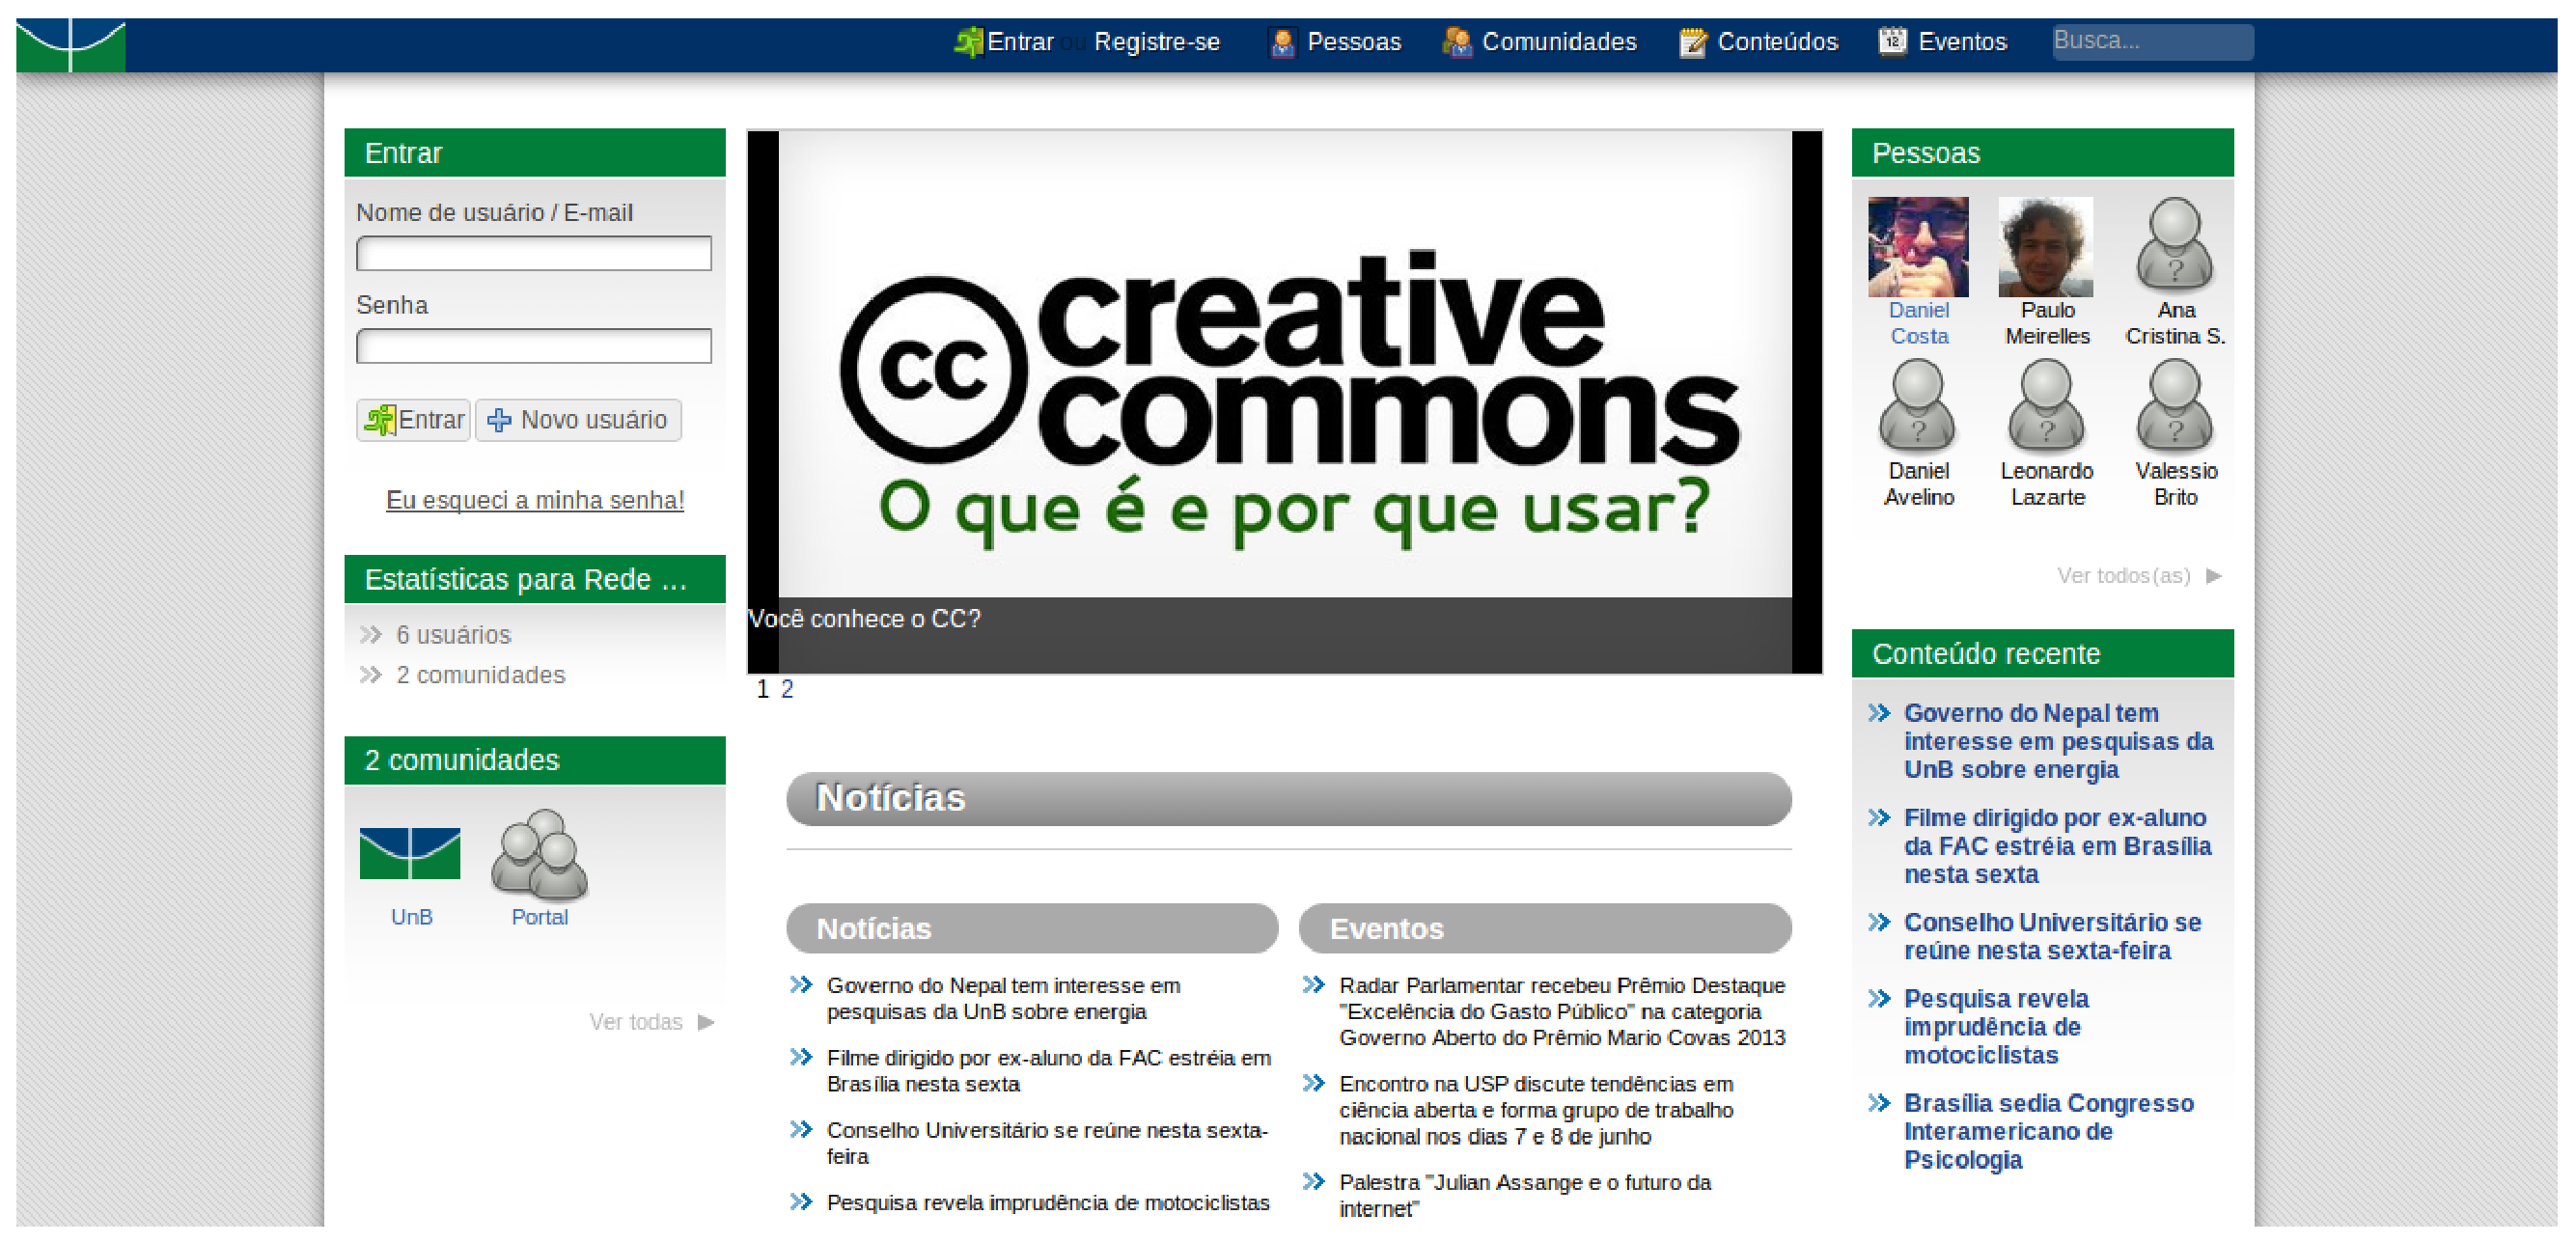
\includegraphics[keepaspectratio=true,scale=0.3]
		{figuras/comunidade.unb.br.eps}
	\caption{Tela inicial da Comunidade UnB}
\end{figure}

O apoio institucional é fundamental para o funcionamento deste trabalho de forma
contínua uma vez que queremos que a Comunidade UnB seja a rede de colaboração
oficial da Universidade. Portanto, pretendemos utilizar este trabalho como um
ponto de partida para formalizar uma proposta de criação de um projeto de
desenvolvimento e manutenção desta rede através da colaboração de alunos
bolsistas. Por exemplo, já foi submetida uma solicitação de bolsas para um projeto
de iniciação científica no edital do ProIC (Projeto de Iniciação científica)
aberto no primeiro semestre de 2013 pelo DPP (Decanato de Pesquisa e Pós-
Graduação) da UnB.

%------------------------------------------------------------------------------%

\subsection{Uso do Noosfero na Disciplina de Manutenção e Evolução de Software}
\label{mes-unb}

Um exemplo do uso de uma rede de colaboração, como ambiente de apoio ao ensino,
pode ser visto no caso da disciplina do curso de Engenharia de Software de
Manutenção e Evolução de Software (MES), ministrada, no primeiro semestre de
2013, pelo professor Paulo Meirelles, na qual eu participei como monitor
voluntário.

A disciplina teve como objetivo permitir com que os
alunos pudessem vivenciar situações reais de desenvolvimento de software ao
exercer atividades de manutenção, seja evolutiva, corretiva, perfectiva ou
qualquer outra forma de manutenção, em projetos de software livre e fez uso de
uma comunidade
~\footnote{Disponível em: \url{http://social.stoa.usp.br/mes-fga-unb/ementa}}
criada na rede de colaboração da USP, o Stoa, como ferramenta de comunicação a ser
utilizado pelo grupo e para a publicação dos resultados dos projetos.
%
A turma foi divida em grupos que selecionaram o projeto, dentro de uma lista
de opções fornecidas pelo professor, no qual desejavam atuar. Foi criado um 
sub-grupo, que funciona como uma comunidade normal, porém vinculada à comunidade
da disciplina, para cada projeto da disciplina. A Figura 4 (\ref{mes-unb})
apresenta a página da ementa da comunidade supracitada. 

\begin{figure}[h]
	\centering
	\label{mes-unb}
		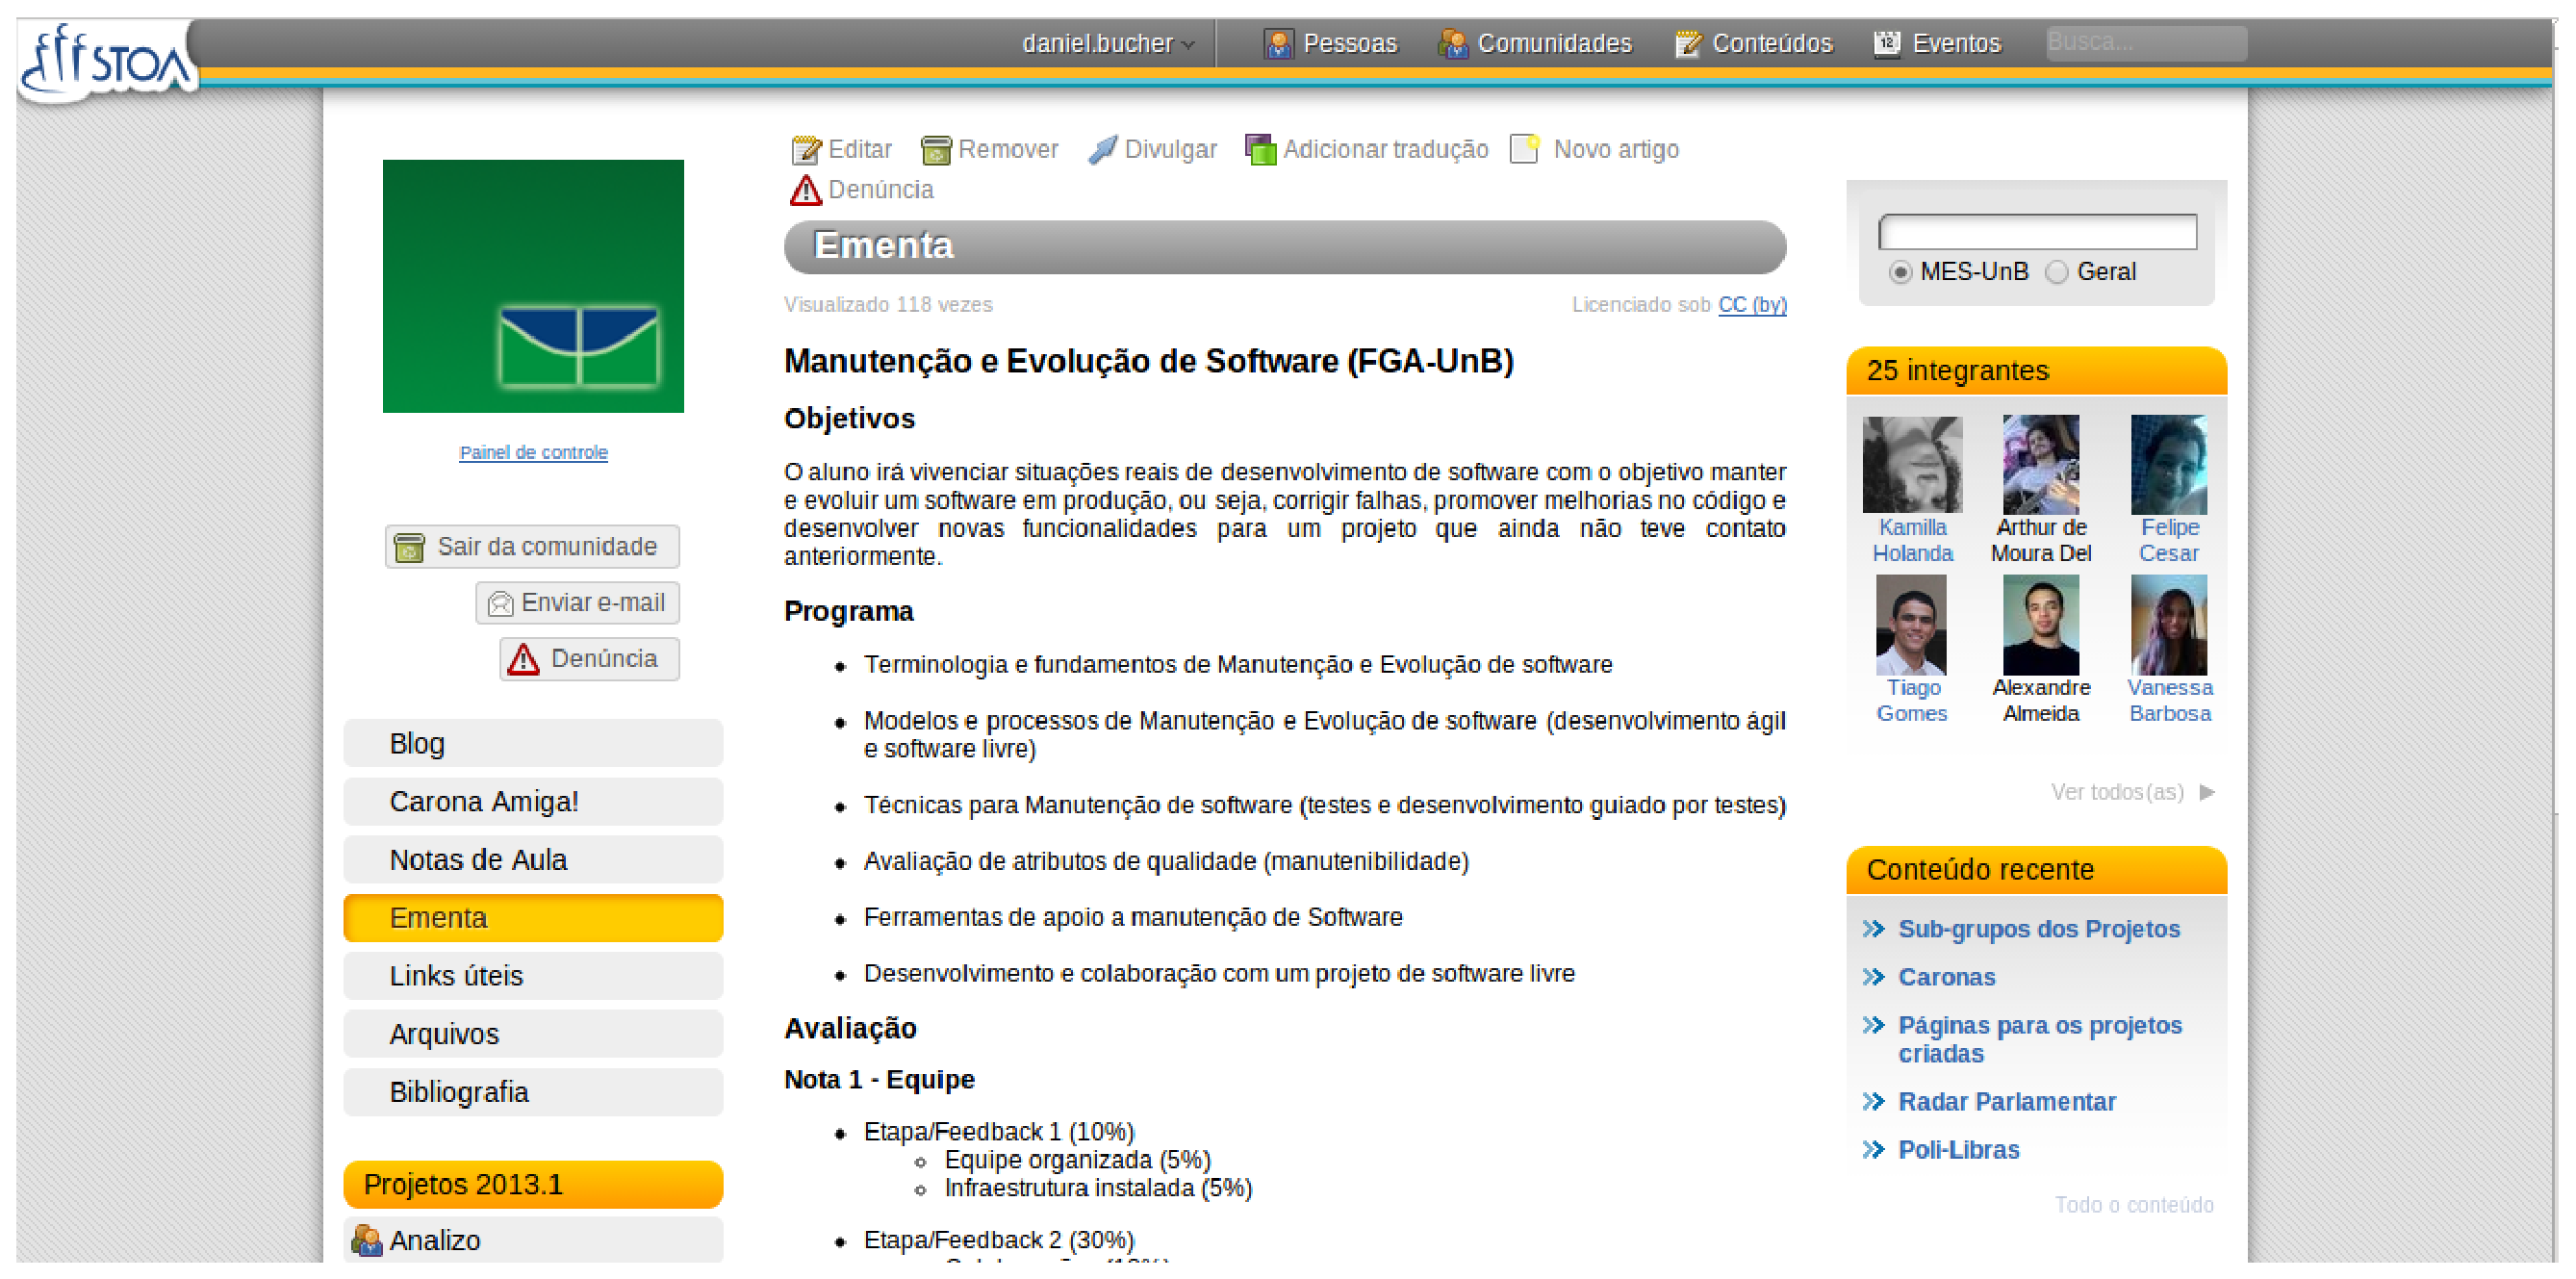
\includegraphics[keepaspectratio=true,scale=0.3]
		{figuras/mes-unb.eps}
	\caption{Comunidade da disciplina de Manutenção e Evolução de Software}
\end{figure}

A Figura 5 (\ref{analizo}) apresenta o \textit{blog} do sub-grupo
criado para o projeto de manutenção na ferramenta Analizo~\footnote{Disponível
em \url{http://social.stoa.usp.br/analizo}}, uma ferramenta livre
para análise estática de código. O grupo optou por utilizar o \textit{blog}
para publicar o progresso do projeto no formato de \textit{release notes} e
retrospectivas dos ciclos de desenvolvimento.

\begin{figure}[h]
	\centering
	\label{analizo}
		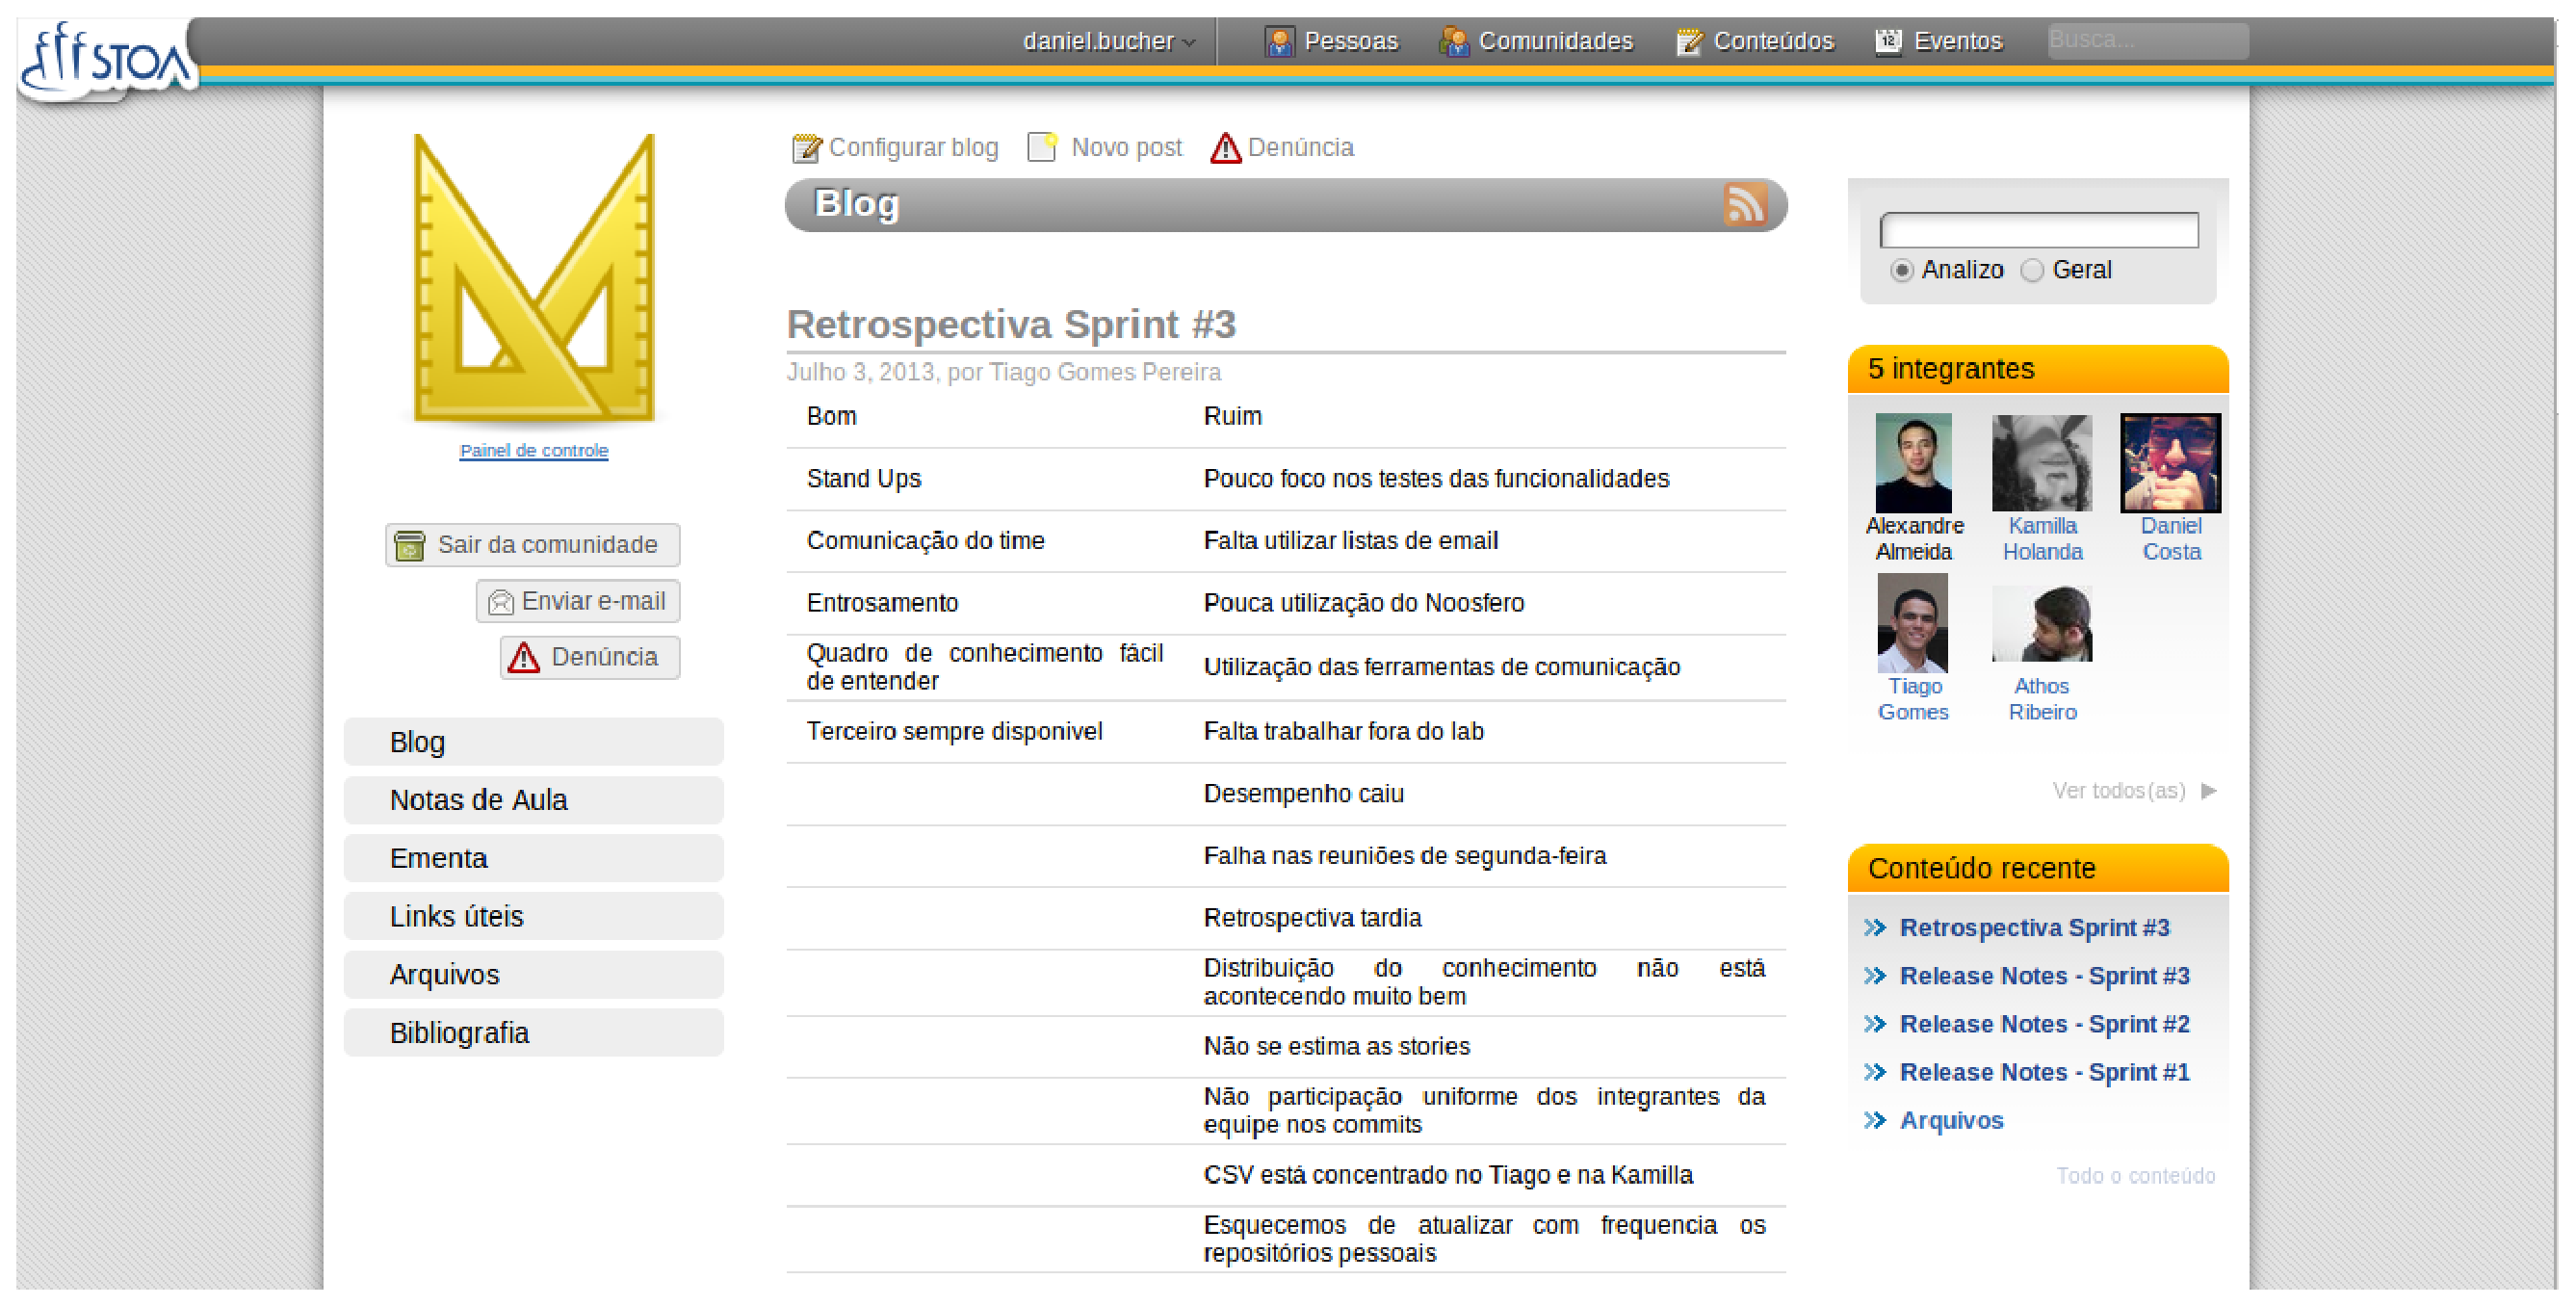
\includegraphics[keepaspectratio=true,scale=0.3]
		{figuras/analizo.eps}
	\caption{Blog do sub-grupo do projeto Analizo da disciplina de MES }
\end{figure}

A comunidade da disciplina de MES foi criada na rede da USP, com consentimento
da administração da mesma, pelo fato de que a rede Comunidade UnB ainda estar
passando por uma fase de desenvolvimento e testes. Pretendemos apresentar
na segunda fase deste trabalho a ser apresentado no segundo semestre de 2013
uma pesquisa de satisfação dos alunos com o uso da plataforma na disciplina e
assim coletar \textit{feedbacks} e propostas de melhorias para a mesma. 

%------------------------------------------------------------------------------%

\section{Levantamento de Requisitos da Comunidade UnB}
\label{requisitos}

Esta seção apresenta os requisitos levantados por nós para a disponibilização
da rede de colaboração da UnB. As sub-seções a seguir apresentam alguns
requisitos funcionais e não funcionais que foram observados, levando
em consideração que a ferramenta deve satisfazer às necessidades de alunos,
professores e funcionários da Universidade e garantir a disponibilidade do
serviço.

%------------------------------------------------------------------------------%
\subsection{Funcionalidades}

As funcionalidades disponíveis no Noosfero, seja em seu \textit{core}
ou através de \textit{plugins} já nos permite fazer uso da plataforma como
um ambiente virtual para a troca de conhecimento através das comunidades e
perfis de usuários, e como portal para departamentos e organizações da
Universidade (\ref{noosfero-section}).
%
A seguir apresentamos algumas funcionalidades que julgamos interessantes
incorporar na Comunidade UnB, através da criação do \textit{plugin} Comunidade-
UnB, para melhorar o uso da mesma em um contexto educacional:

	\begin{enumerate}
		\item Autenticação via base de dados da UnB:
		Estamos pesquisando a existência de uma base de dados que possa
		ser utilizada para a autenticação na rede via matrícula. Desta forma,
		todos os alunos, professores e funcionários da UnB já possuiriam
		cadastro na rede e precisariam apenas personalizar seu perfil.
		\item Integração com os diversos Moodles da Universidade:
		A integração ocorreria no sentido que, ao criar um novo curso no
		Moodle, uma comunidade seria automaticamente criada na Comunidade
		UnB. Atualmente a UnB possui uma instância de Moodle para cada
		campus.
	\end{enumerate}

Outras possíveis funcionalidades serão coletadas durante uma pesquisa com os
alunos que utilizaram o Stoa durante a disciplina de MES.

%------------------------------------------------------------------------------%
\subsection{Requisitos Não-funcionais}

Em relação aos requisitos não funcionais, separamos algumas características que
julgamos necessárias para o bom funcionamento da Comunidade UnB, principalmente
em relação à disponibilidade, performance e segurança do sistema.

É importante para o sucesso da Comunidade UnB que esta permaneça disponível
mesmo durante picos de acesso estimados em até 30 mil usuários simultâneos,
que dá aproximadamente 75\% do total de candidatos a usuários da Universidade
que possui atualmente 2.445 professores, 2.630 técnicos-administrativos
e 28.570 alunos regulares e 6.304 de pós-graduação, totalizando de 39.949
\cite{unbInstituicao}. Como explicado na seção \ref{noosfero-section}, o Noosfero
utiliza o \textit{web-server} Apache como um servidor de \textit{proxy} reverso
que realizar o balanceamento de carga entre as diversas instâncias do Thin,
configuradas durante a instalação, sendo que são recomendadas a configuração de
duas instâncias por núcleo de processador presentes na máquina que está
hospedando o sistema.
%
Estimamos que necessitaríamos de 8 instâncias do Thin
para manter um nível de performance aceitável durante picos de acesso, o que
necessitaria de uma máquina com pelo menos 4 núcleos de processamento para
hospedar o sistema. No entanto, essa estimativa foi realizada com base em
depoimentos de usuários destas tecnologias e faz-se necessária a execução de
um \textit{benchmark} mais específico para podermos definir estes parâmetros com
uma precisão maior.

Quanto à questão de segurança de acesso, o ideal é que a autenticação seja
realizada através de um serviço ou uma base de dados disponibilizada pelo CPD
(Centro de Informática) e que seja utilizada uma camada de SSL/TLS (Secure Socket
Layer e Transport Layer Security) através do protocolo HTTPS (Hypertext Transfer
Protocol Secure) para acesso à Comunidade UnB. As permissões de acesso das
comunidades e seu conteúdo podem ser configuradas através do painel de controle
das mesmas. Atualmente estamos investigando a possibilidade de utilizarmos a
base de dados o MatriculaWeb
~\footnote{\url{https://matriculaweb.unb.br/matriculaweb/}}, serviço de matrícula
da UnB para autenticar no sistema. Outra possibilidade seria utilizar as bases
de dados das diversas instâncias de Moodle existente na Universidade.
	

%------------------------------------------------------------------------------%

Outro aspecto importante que devemos levar em consideração é a adequação da
Comunidade Unb ao padrão de identidade visual da UnB.
A identidade visual da rede foi adaptada em cima do tema~\footnote{Temas são
compostos por aquivos de \textit{layout}, em rhtml e CSS, que definem os aspectos
visuais de uma instância do Noosfero. Os temas podem ser alterados pela interface
administrativa da instância.} do Stoa, que é disponibilizada em um repositório
público, para se enquadrar no padrão da UnB.
%
O \textit{layout} atual utiliza predominantemente as duas cores-padrão definidas
no Manual de Identidade Visual da Universidade\cite{visualUnB}, o Azul UnB
(Pantone 654) e o Verde UnB (Pantone 348). Na Figura 3 (\ref{comunidade-unb})
podemos ver uma versão temporária do \textit{layout} desenvolvida por nós.

%------------------------------------------------------------------------------%

\subsection{Federação}

A transição do Noosfero para uma rede social federada é essencial para a criação
de um ecosistema de redes de colaboração que comunicam entre si. A federação
consiste na habilidade de redes diferentes de conversarem entre si de forma que
um usuário da rede Comunidade UnB poderia receber atualizações de uma comunidade
em outra rede baseada em Noosfero ou em qualquer outra ferramenta que implemente
o mesmo protocolo de federação, através de regras pré-acordadas.

Em princípio, a estrutura para redes federadas proposta para a plataforma Noosfero
consistia em um padrão aberto, chamado OStatus
~\footnote{\url{http://www.w3.org/community/ostatus/}}, que foi proposto
por Evan Prodomou para ser utilizado pelo StatusNet~\footnote{\url{
http://status.net/}}, um servidor  \textit{open-surce} para
\textit{microblogging} escrito em PHP.
%
O OStatus foi construído com base no padrõe para criação de \textit{feeds},
Atom~\footnote{\url{http://www.atomenabled.org/}} e no protocolo PuSH
~\footnote{\url{https://code.google.com/p/pubsubhubbub/}}(PubSubHubbub).
O funcionamento do OStatus pode ser resumido da seguinte forma:
os \textit{sites} produzem atualizações no formato de \textit{feeds} através
do padrão Atom e utilizam o protocolo PuSH para enviar estas atualizações
para outros \textit{sites} \\
\cite{OStatusBasics}.
%
Posteriormente, OStatus passou a ser desenvolvido como um grupo de trabalho
da W3C e estava no caminho para se tornar um padrão oficial. 

No entanto, em dezembro de 2013, Prodomou declarou que estava desenvolvendo
um novo projeto chamado \textit{pump.io} quer iria substituir o StatusNEt
~\footnote{\url{http://status.net/2012/12/18/upcoming-changes-in-the-status
-net-service}} e que utilizará um novo protocolo para a federação chamado
Activity Streams~\footnote{\url{http://activitystrea.ms/}} baseado em JSON.
A adoção de um destes dois protocolos está sendo discutida pela comunidade do
Noosfero, mas já existe uma previsão para se começar a implementar a federação
para o mesmo, ainda em 2013. Parte deste trabalho consiste em colaborar com esta
implementação.
%------------------------------------------------------------------------------%

\section{Cronograma de Trabalho}

O cronograma para o trabalho realizado neste TCC é apresentado na Tabela 1 
(\ref{cronograma}). As atividades planejadas são:

\begin{enumerate}
	\item Configuração de ambiente de desenvolvimento e testes.
	\item Pesquisa e desenvolvimento de um \textit{layout} baseado nos
	padrões de identidade visual da UnB.
	\item Pesquisa de satisfação dos alunos da disciplina de MES 2013.1 e
	estudo exploratório com alunos de 2013.2.
	\item Desenvolvimento da autenticação da Comunidade UnB.
	\item Colaboração no desenvolvimento do protocolo de federação
	selecionado.
	\item Desenvolvimento de novas funcionalidades de acordo com um
	levantamento de requisitos através das pesquisas e estudos exploratórios
	planejados.
	\item Disponibilização da Comunidade UnB em ambiente de homologação.
	\item Escrita do TCC
	\item Escrita e submissão de artigo para um workshop/conferência de
	Informática na Educação (ou similar).
\end{enumerate}

\begin{table}[h]
	\centering
	\label{cronograma}
	
	\begin{tabular}{|c|c|c|c|c|c|c|}
		\hline
		\textbf{Atividades}	& \textbf{Ago 2013}	& \textbf{Set 2013}
		& \textbf{Out 2013}	& \textbf{Nov 2013}	& \textbf{Dez 2013}
		& \textbf{Jan 2014}	\\
		\hline\hline
		
		\hline
		1	& • 	&	&	&	&	&	\\
		\hline

		\hline
		2	& •	& •	&	&	&	&	\\
		\hline

		\hline
		3	& •	&	&	&	&	&	\\
		\hline

		\hline
		4	&	&	& •	&	&	&	\\
		\hline

		\hline
		5	& 	&	& •	& •	& •	&	\\
		\hline

		\hline
		6	& 	&	& •	& •	& •	&	\\
		\hline

		\hline
		7	& 	&	& 	& 	& •	&	\\
		\hline

		\hline
		8	& 	&	& 	& • 	& •	&	\\
		\hline

		\hline
		9	& 	&	& 	& 	& 	& •	\\
		\hline
	\end{tabular}

	\caption{Cronograma}
\end{table}
%------------------------------------------------------------------------------%
